\titleframe{Results}

\mframe{Ground State Energy}{Number of electrons: $N=2$. Frequency: $\omega$.}{
\begin{table}
	%\caption{$N=2$}
	\begin{tabularx}{\textwidth}{lR{1.25cm}R{1.25cm}R{1.4cm}R{1.4cm}R{1.2cm}R{1.cm}} 
		\toprule
		$\omega$ & RBM & RBM+SJ & RBM+PJ & VMC & HF \footnote{Computation of the Hartree-Fock limit by \citeauthor{mariadason_quantum_2018}, \citeyear{mariadason_quantum_2018} \cite{mariadason_quantum_2018}.} & Exact \footnote{Semi-analytical ground state energy calculated by \citeauthor{taut_two_1993}, \citeyear{taut_two_1993} \cite{taut_two_1993}.} \\
		\midrule \\
		1/6 & 0.7036(1) & 0.67684(7) & 0.66715(6) & 0.66710(1) & 0.768675 & 2/3 \\ 
		0.28 & 1.07050(4) & 1.03470(7) & 1.021668(7) & 1.02192(1) & 1.14171 \\
		1 & 3.0803(2) & 3.02108(5) & 2.999587(5) & 2.99936(1) & 3.16190 & 3 \\
		\bottomrule
	\end{tabularx}
\end{table}
}

\note{The first results that I would like to present, is the ground state energy of quantum dots with two electrons and some selected frequencies. We look at the frequencies $\omega=1/6$ and 1 because there exist exact energies for these two systems. Additionally, we present the frequency $\omega=0.28$. We see here that the RBM ansatz, in the first column, provides energies not very far from the analytical energies in this last column. They are also lower than the Hartree-Fock limit, which is interesting as the Hartree-Fock algorithm attempts to find the optimal Slater determinant without Jastrow factors. When we add more intuition in the form of a simple Jastrow factor, the energy drops further towards the exact energy. The RBM+PJ ansatz is totally on pair with the VMC ansatz, and for $\omega=0.28$ the ansatz provides a significantly lower energy. This is also the case for other frequencies that we have tested, and indicates that the RBM+PJ ansatz is able to obtain a better estimate of the ground state energy than the standard VMC ansatz. }

\mframe{Ground State Energy}{Number of electrons: $N=20$. Frequency: $\omega$.}{
\begin{table}
	%\caption{$N=20$}
	\begin{tabularx}{\hsize}{lR{1.25cm}R{1.25cm}R{1.3cm}R{1.4cm}R{1.cm}R{1.4cm}} \\
		\toprule
		$\omega$ & RBM & RBM+SJ & RBM+PJ & VMC & HF \footnote{Computation of the Hartree-Fock limit by \citeauthor{mariadason_quantum_2018}, \citeyear{mariadason_quantum_2018} \cite{mariadason_quantum_2018}.} & DMC \footnote{Ground state energy estimate using the diffusion Monte Carlo method. By \citeauthor{hogberget_quantum_2013}, \citeyear{hogberget_quantum_2013} \cite{hogberget_quantum_2013}.} \\
		\midrule \\
		0.1 & 30.824(2) & 30.567(3) & 30.1553(9) & 30.0403(2) & 31.1902 & 29.9779(1) \\ 
		%0.28 & 63.788(4) & 62.786(3) & 62.148(1) & 63.5390 & 62.0755(7) & 61.9268(1) \\
		%0.5 & 96.410(1) & 94.920(4) & 94.104(1) & 95.7328 & 94.0433(9) & 93.8752(1) \\
		1.0 & 159.428(3) & 156.816(4) & 156.104(1) & 155.8900(4) & 158.004 & 155.8822(1) \\ 
		\bottomrule
	\end{tabularx}
\end{table}
}

\note{We also investigate quantum dots with 20 electrons and frequencies $\omega=0.1$ and 1.0. For these systems, we do not have analytically energy, but we use the diffusion Monte Carlo energy as reference, which is believed to be more or less exact. What we see is that the RBM ansatz again is not far from the reference, but for high frequency the energy is larger than the Hartree-Fock limit. This illustrates that RBM is better at modelling correlations than Hartree-Fock. The reason why the energy is larger than HF for frequency $\omega=1.0$, might be that it has not fully converged. This ansatz is equipped with 860 variational parameters, making it an optimization problem. }

\mframe{Energy distribution}{Number of electrons: $N=20$. Frequency: $\omega$.}{
	Ratio between the kinetic energy, $\langle\hat{T}\rangle$, and the total potential energy, $\langle\hat{V}\rangle$.
	\begin{figure}
		\centering 
		\begin{tikzpicture}

\begin{axis}[
legend cell align={left},
legend style={at={(0.9,0.1)}, anchor=south east, draw=white!80.0!black},
title style={yshift=-1.5ex},
%tick align=outside,
tick pos=both,
x grid style={white!69.01960784313725!black},
xlabel={\(\displaystyle \omega\)},
width=8cm,
height=6cm,
xmajorgrids,
xmin=-0.4895, xmax=10.4995,
xtick style={color=black},
y grid style={white!69.01960784313725!black},
ylabel style={rotate=-90.0},
ylabel={\(\displaystyle \frac{\langle\hat{T}\rangle}{\langle\hat{V}\rangle}\)},
ymajorgrids,
%ymin=-0.03, ymax=0.7,
ytick style={color=black}
]
\addplot [thick, color0]
table {%
	0.01 0.0202855736090596
	0.1 0.0558188176084186
	0.28 0.0748673013733255
	0.5 0.092181964299863
	1 0.120447174205168
	2 0.191577362501107
	3 0.2257693437
	5 0.263982205508037
	10 0.278872126802915
};
\addlegendentry{RBM}
\addplot [thick, color1]
table {%
	0.01 0.0224807471735212
	0.1 0.0510365183964855
	0.28 0.0535270823545204
	0.5 0.0761996706229769
	1 0.108428284656055
	2 0.17366909653192
	3 0.19307880632568
	5 0.260942252768941
	10 0.332349732889548
};
\addlegendentry{RBM+SJ}
\addplot [thick, color2]
table {%
	0.01 0.0198390540318607
	0.1 0.0550696242390316
	0.28 0.0812272164373049
	0.5 0.0960548685344326
	1 0.120346512979882
	2 0.152555093728466
	3 0.20363356015151
	5 0.286590458917023
	10 0.373618884667807
};
\addlegendentry{RBM+PJ}
\addplot [thick, color3]
table {%
	0.01 0.0164511376657391
	0.1 0.0430938843433643
	0.28 0.067074638154502
	0.5 0.0907330085826954
	1 0.121087634122869
	2 0.176534004132603
	3 0.20481414099371
	5 0.307872099467483
	10 0.330233868695407
};
\addlegendentry{VMC}
\end{axis}
\end{tikzpicture}
		%\caption{$N=20$}
	\end{figure}
}

\note{We also look at the distribution between kinetic energy and total potential energy. Keep looking at quatum dots with 20 electrons, we see that the potential energy dominates over the potential energy when the frequency gets low. Also, the various ansätze differ more for high frequencies. }

\mframe{One-body density}{Number of electrons: $N=20$. Frequency: $\omega=1.0$.}{
	\begin{figure}
		\centering
		\captionsetup[subfigure]{labelformat=empty}
		\subfloat{\raisebox{1cm}{\rotatebox[origin=t]{90}{RBM}}}\hspace{0.cm}
		\subfloat{{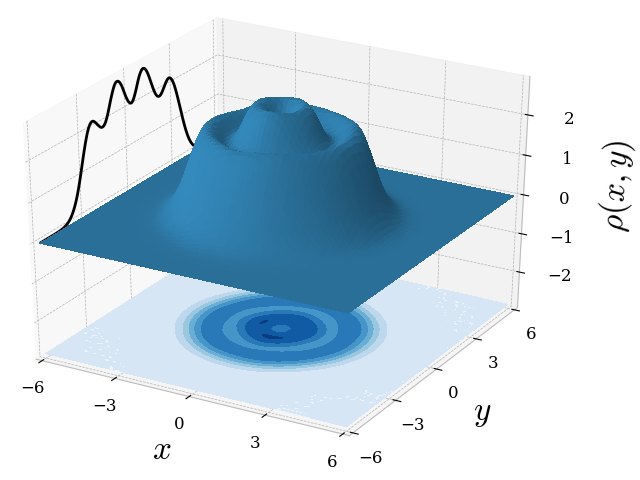
\includegraphics[width=3cm]{../plots/int1/onebody2/2D/20P/1.000000w/RBM_ADAM_MC1048576.png}}}\hspace{0.5cm}
		\subfloat{\raisebox{1cm}{\rotatebox[origin=t]{90}{RBM+SJ}}}\hspace{0.cm}
		\subfloat{{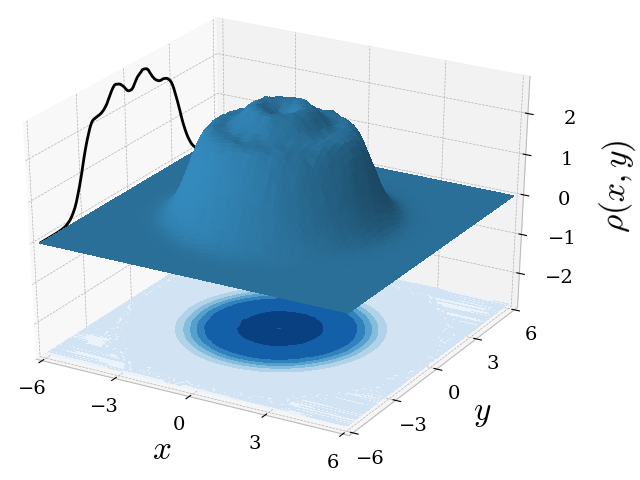
\includegraphics[width=3cm]{../plots/int1/onebody2/2D/20P/1.000000w/RBMSJ_ADAM_MC1048576.png}}}\\
		\subfloat{\raisebox{1cm}{\rotatebox[origin=t]{90}{RBM+PJ}}}\hspace{0.cm}
		\subfloat{{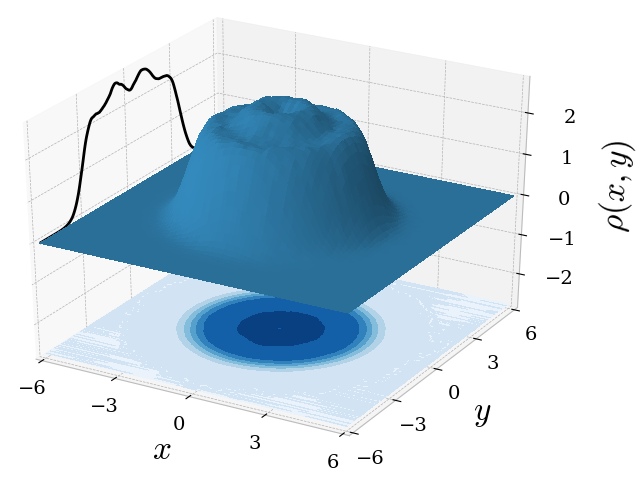
\includegraphics[width=3cm]{../plots/int1/onebody2/2D/20P/1.000000w/RBMPJ_ADAM_MC1048576.png}}}\hspace{0.5cm}
		\subfloat{\raisebox{1cm}{\rotatebox[origin=t]{90}{VMC}}}\hspace{0.cm}
		\subfloat{{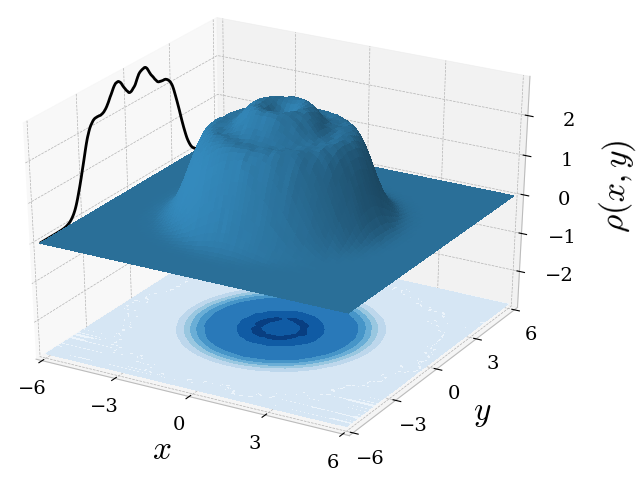
\includegraphics[width=3cm]{../plots/int1/onebody2/2D/20P/1.000000w/VMC_ADAM_MC1048576.png}}}
		%\caption{$N=20$, $\omega=1.0$}
	\end{figure}
}

\note{Now, we look at the one-body density provided by the various ansätze. We observe that all the ansätze with a Jastrow factor, i.e. RBM+SJ, RBM+PJ and VMC, provide very similar density profiles, while RBM provides more distinct peaks. It looks like the RBM ansatz manages to find the same extrema as the other ansätze, but determines another density there. }

\mframe{Two-body density}{Number of electrons: $N=20$. Frequency: $\omega=1.0$.}{
	\begin{figure}
		\centering
		\captionsetup[subfigure]{labelformat=empty}
		\subfloat{\raisebox{1cm}{\rotatebox[origin=t]{90}{RBM}}}\hspace{0.cm}
		\subfloat{{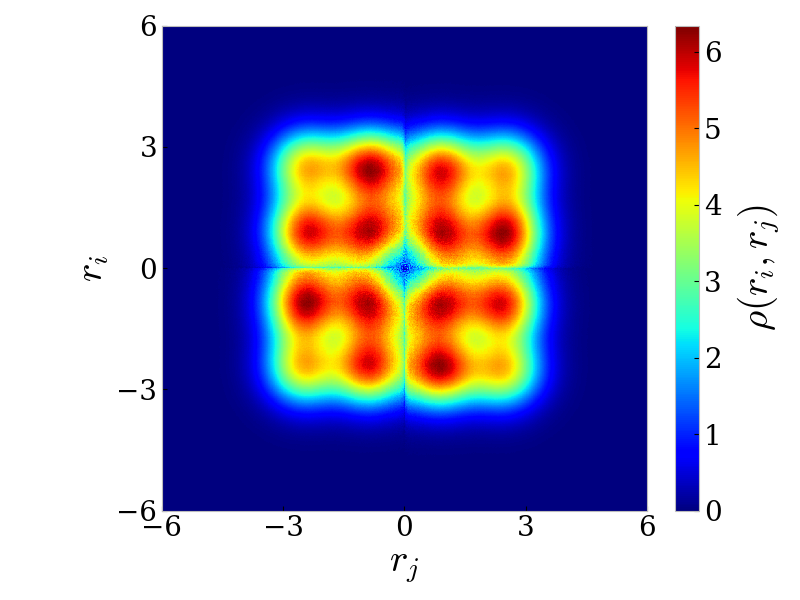
\includegraphics[width=3cm]{../plots/int1/twobody/2D/20P/1.000000w/RBM_ADAM_MC1048576.png}}}\hspace{0.5cm}
		\subfloat{\raisebox{1cm}{\rotatebox[origin=t]{90}{RBM+SJ}}}\hspace{0.cm}
		\subfloat{{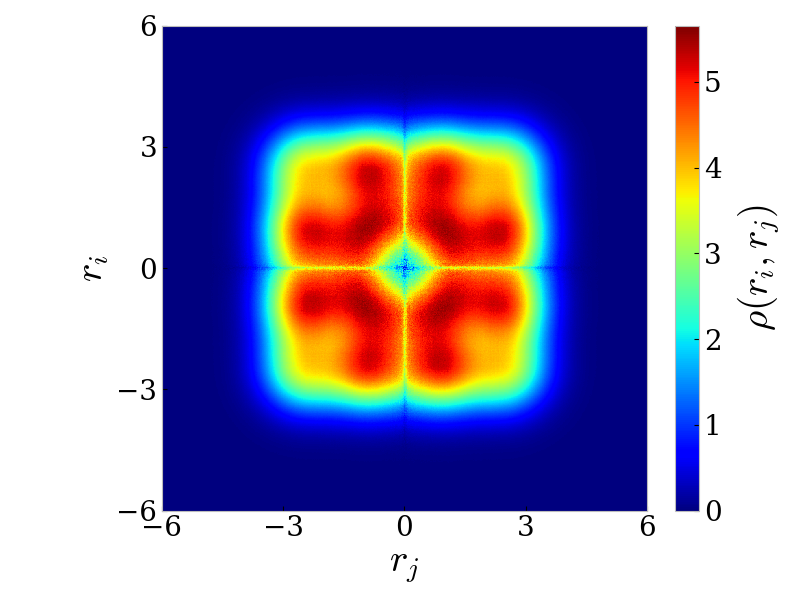
\includegraphics[width=3cm]{../plots/int1/twobody/2D/20P/1.000000w/RBMSJ_ADAM_MC1048576.png}}}\\
		\subfloat{\raisebox{1cm}{\rotatebox[origin=t]{90}{RBM+PJ}}}\hspace{0.cm}
		\subfloat{{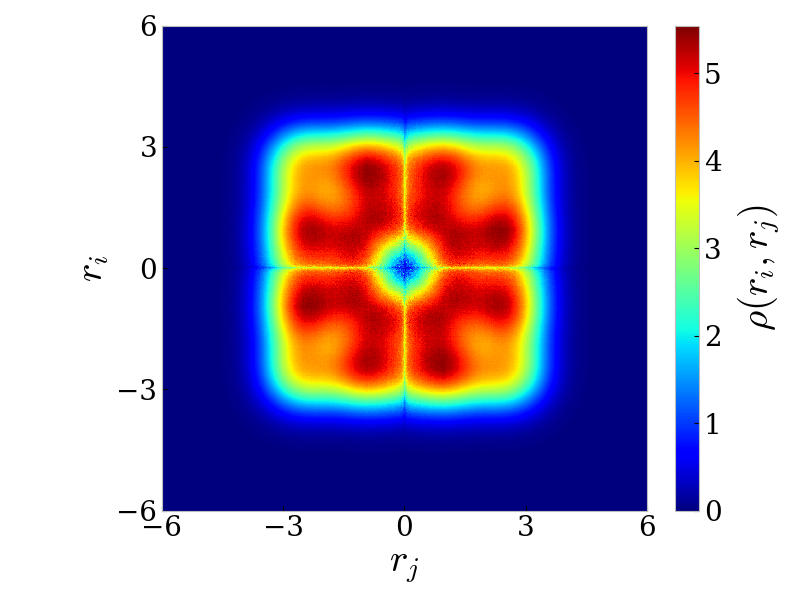
\includegraphics[width=3cm]{../plots/int1/twobody/2D/20P/1.000000w/RBMPJ_ADAM_MC1048576.png}}}\hspace{0.5cm}
		\subfloat{\raisebox{1cm}{\rotatebox[origin=t]{90}{VMC}}}\hspace{0.cm}
		\subfloat{{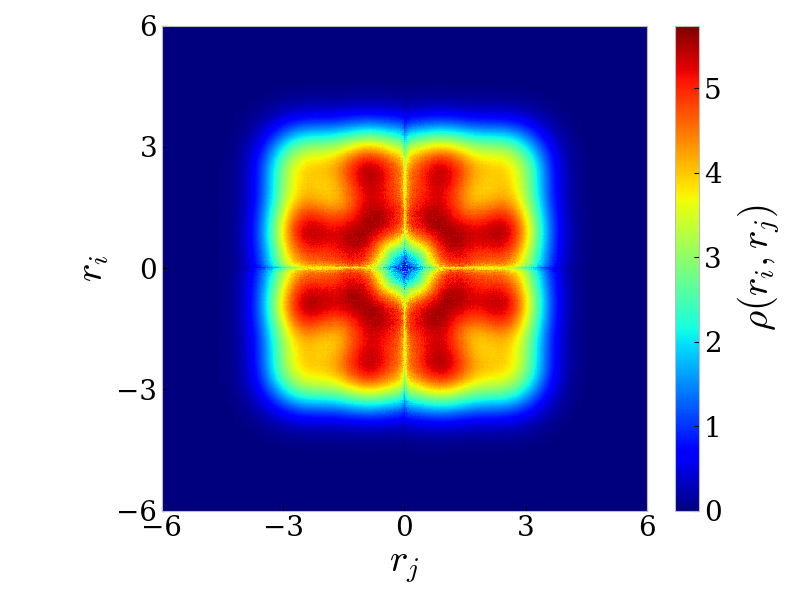
\includegraphics[width=3cm]{../plots/int1/twobody/2D/20P/1.000000w/VMC_ADAM_MC1048576.png}}}
		%\caption{$N=20$, $\omega=1.0$}
	\end{figure}
}

\note{We have also studied the two-body density, which makes us able to study the electron-electron correlations in more detail. A similar phenomenon as we saw for the one-body density can be observed in the two-body density. RBM provides more distinct peaks than its fellow ansätze. }

\mframe{Low-frequency dots}{Number of electrons: $N$. Frequency: $\omega=0.1$.}{
	\begin{figure}
		\centering
		\captionsetup[subfigure]{labelformat=empty}
		\subfloat{\raisebox{1cm}{\rotatebox[origin=t]{90}{RBM}}}\hspace{0.1cm}
		\subfloat{{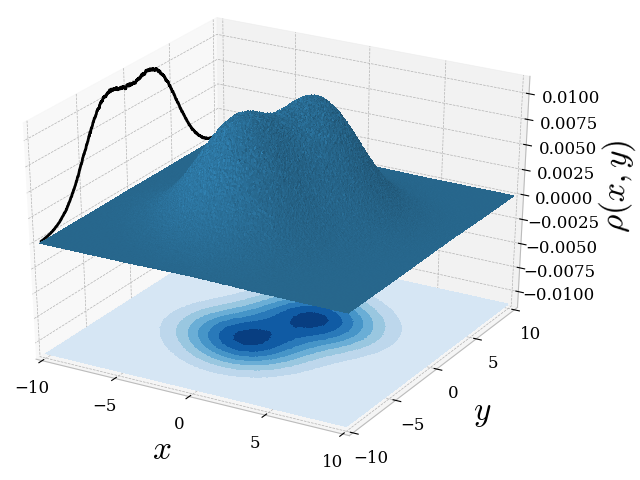
\includegraphics[width=3cm]{../plots/int1/onebody2/2D/2P/0.100000w/RBM_ADAM_MC1048576.png}}}\hspace{-0.cm}
		\subfloat{{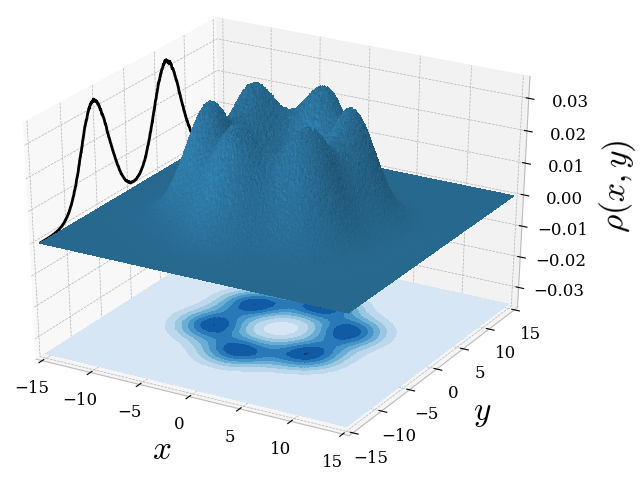
\includegraphics[width=3cm]{../plots/int1/onebody2/2D/6P/0.100000w/RBM_ADAM_MC1048576.png}}}\hspace{-0.cm}
		\subfloat{{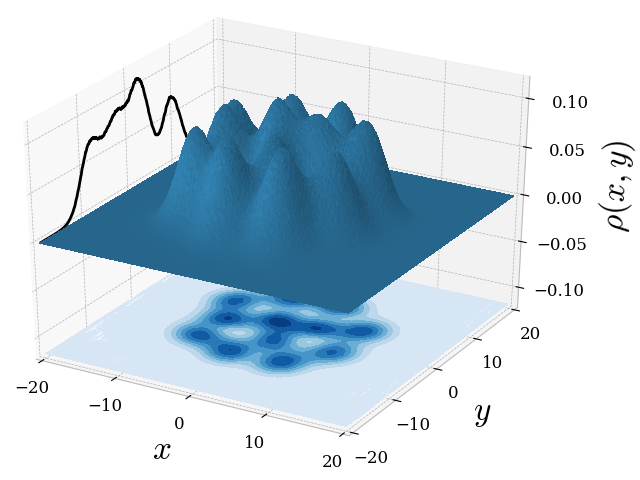
\includegraphics[width=3cm]{../plots/int1/onebody2/2D/12P/0.100000w/RBM_ADAM_MC1048576.png}}}\\ [-0.cm]
		
		\subfloat{\raisebox{1cm}{\rotatebox[origin=t]{90}{VMC}}}\hspace{0.1cm}
		\subfloat[$N=2$]{{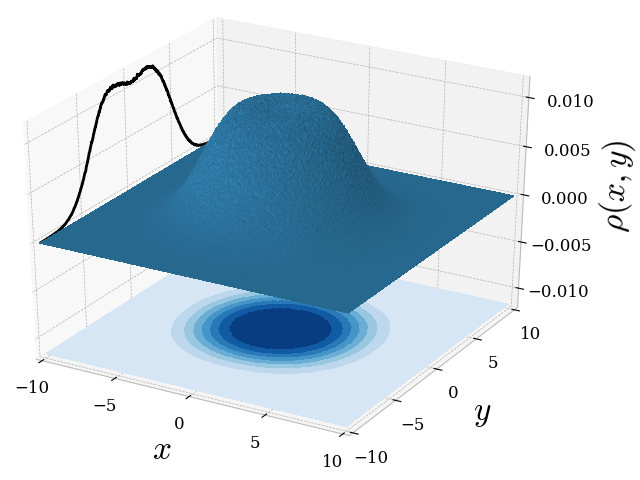
\includegraphics[width=3cm]{../plots/int1/onebody2/2D/2P/0.100000w/VMC_ADAM_MC1048576.png}}}\hspace{-0.cm}
		\subfloat[$N=6$]{{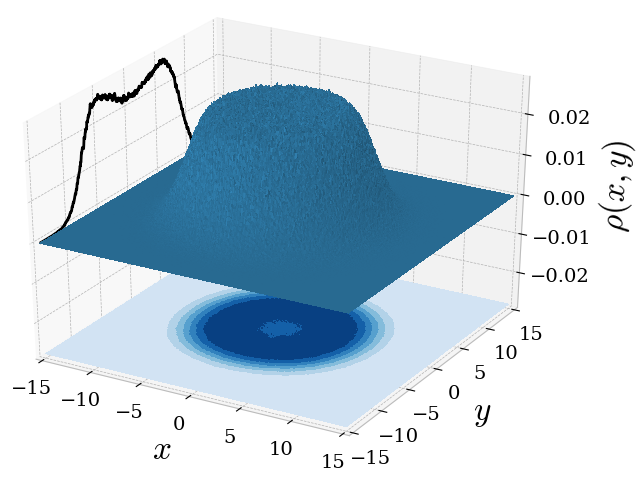
\includegraphics[width=3cm]{../plots/int1/onebody2/2D/6P/0.100000w/VMC_ADAM_MC1048576.png}}}\hspace{-0.cm}
		\subfloat[$N=12$]{{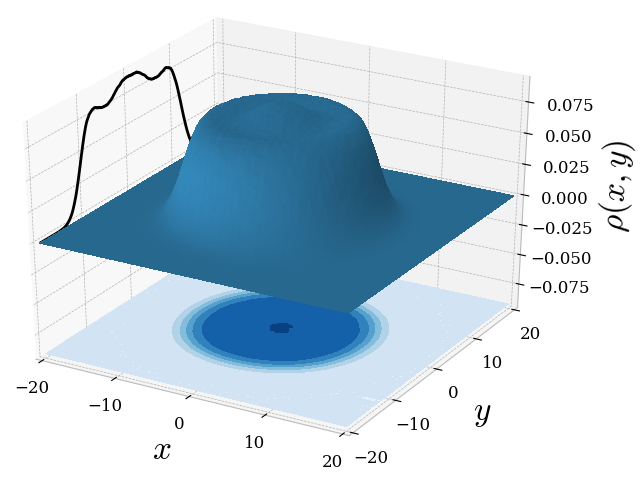
\includegraphics[width=3cm]{../plots/int1/onebody2/2D/12P/0.100000w/VMC_ADAM_MC1048576.png}}}
		%\caption{$\omega=0.1$}
	\end{figure}
}

\note{We now move on to quantum dots with frequency $\omega=0.1$. When comparing the RBM ansatz and the VMC ansatz, we see that the two ansätze give very different one-body density profiles. Apparently, the RBM ansatz provides an equal number of peaks as there are electrons, implying very localized particle positions. What is interesting, is that the energy for the respective methods are quite similar. This indicates that the energy itself might not be the best way to decide whether an ansatz is good or not. }

\mframe{Computational Cost}{Number of electrons: $N$.}{
	\begin{figure}
		\centering 
		% This file was created by matplotlib2tikz v0.7.4.
\begin{tikzpicture}[scale=0.9]

\begin{axis}[name=2D, xlabel=$N$, ylabel={CPU-time [s]}, grid=major, legend pos=north west, xtick=data] 
\addplot[color=color1,mark=oplus*, dashed] coordinates { 
	(2,6.05)
	(6,11.25)
	(12,20.53) 
	(20,38.99) 
	(30,73.73) 
	(42,130.49) 
	(56,213.47)
	(72,360.22)
	(90,856.84) }; 
\addlegendentry{RBM};

\addplot[color=color2,mark=oplus*, dash dot] coordinates { 
	(2,7.12) 
	(6,14.07) 
	(12,28.42) 
	(20,63.27) 
	(30,122.93) 
	(42,199.60)
	(56,349.22)}; 
\addlegendentry{RBM+SJ};

\addplot[color=color3,mark=oplus*, dotted] coordinates { 
	(2,7.26)
	(6,13.50)
	(12,27.68)
	(20,57.09) 
	(30,119.17) 
	(42,212.53) 
	(56,382.13) }; 
\addlegendentry{RBM+PJ};

\addplot[color=color0,mark=oplus*] coordinates { 
	(2,5.11)
	(6,10.51)
	(12,20.85) 
	(20,41.20) 
	(30,76.26) 
	(42,137.39) 
	(56,230.63)
	(72,355.81)
	(90,544.03) }; 
\addlegendentry{VMC};
\end{axis}
\end{tikzpicture}
	\end{figure} 
}

\note{In the end, we will also compare the computational cost of the various methods. From the curves, we see that the RBM and VMC ansätze are pairwise the computationally cheapest methods and RBM+SJ and RBM+PJ are the most computational intensive ones. This is no big surprise, as the two latter methods contain both a neural network and a Jastrow factor. We also see that the cost of the RBM ansatz explodes for very large systems. This is probably because the ansatz then contains around 15,000 variational parameters, while the VMC ansatz contains two variational parameters. }